% !TEX root = ../thesis.tex
%
\chapter{Tangible User Interfaces fostering Computational Thinking skills}
\label{sec:tapas}

\section{Introduction}
In the past few years our lives have been flooded by a multitude of new ubiquitous computing systems, including multi-touch-enabled smartphones, voice-controlled virtual personal assistants, gesture-recognition devices, and so on. These systems all feature a revolutionary emerging interaction paradigm evolved over the past two decades and founded on the most basic and innate human interaction capabilities, such as touch, vision and speech, known as \acp{NUI}. Unlike the more traditional interfaces based on artificial control mechanisms such as the mouse and keyboard, a \ac{NUI} relies only on a user being able to carry out simple and arguably easily discoverable motions to control the on-screen application and manipulate its content.

\acp{TUI} represent one of the first successful attempts at developing a \ac{NUI}, inspired by the physical world, thus allowing users to interact with the digital system in the same way as they would interact with a physical object, providing data and computational power with a physical shape \citetemp{Ishii:1997gy}. By taking advantage of our innate dexterity for object manipulation, \acp{TUI} have proven to be very effective in making highly abstract activities such as programming more direct and accessible. In addition, there are interesting preliminary results linking the usage of tangible tools with increased ability to model abstract concepts \cite{McNerney:2004jc,Horn:2009be}; 
these findings suggest that physical manipulation acts as a scaffold between the real and digital, enhancing  Computational Thinking skills \cite{Wang:2014jy}.

Nevertheless, it is not just the input modality that makes an interface natural: it has to leverage each user's capabilities and meet her needs while fitting the current task and context demands. The design of innovative digital systems like Pervasive Displays has indeed followed many principles \cite{Wigdor:2011:BNW:1995309} with the aim of making interactions as \emph{natural} as possible, in order to support their appropriation and widespread use; these systems are composed of various-sized displays supporting a many-to-many interaction modality and allowing ``many people to interact with the same public screens simultaneously'' \cite{Terrenghi:2009kr}.

In recent years, thanks to the newly available technologies and the intuitive interaction capabilities of Pervasive Displays, they have spread around public areas such as museums, tourist information centers, universities, shopping malls and various other urban locations \cite{Bellucci:2014jj,Ardito:2015gq}. A new trend has recently emerged within Pervasive Displays research, namely to design large and long-term deployments outside traditional controlled laboratory settings with no researchers' supervision, in other words \emph{in-the-wild}. These studies evaluate artifacts in their habitual use context within people's lives; this means observing and recording what people do with them and how their usage changes over time \cite{Crabtree:2013coba}.

Yet, long term deployments of Pervasive Displays present two main drawbacks \cite{RealWorld}:
\begin{enumerate*}[label=(\arabic*)]
	\item their setup and daily operational activities are expensive, and
	\item users and site managers tend to lose interest in their usage and maintenance over time. Even if at first it is easy to advertise the provided benefits through articles and papers presenting similar success stories, problems start to surface when the initial buzz and enthusiasm (novelty) wears off and managers have to carry out the daily maintenance tasks. In addition, keeping these systems interesting over time by constantly providing them with fresh content has proven to be particularly challenging \cite{Memarovic:2013:PLF:2491500.2491505}.
\end{enumerate*}

To solve these problems, Hosio et al. \cite{RealWorld} suggest that allowing a degree of appropriation when designing Pervasive Displays might enable all the stakeholders to understand how such systems could relate to the ordinary activities they often take for granted, leading to a more sustained and prolonged use. Moreover, their public and moderated nature does not allow the provision of a broad set of general purpose and unfixed features, because users' interests and needs are commonly heterogeneous and continuously evolving. Thus, Pervasive Displays need to be adapted to all the different users' needs and repurposed as those needs shift over time to promote a more serendipitous and prolonged usage.

We then argue that \ac{EUD} could be effective in enabling users to adapt and repurpose Pervasive Displays without any intervention of site managers. In addition, in order to provide a coherent and immersive user experience, users need to be able to carry out this activity in the most natural way possible, ideally in the same way they already interact with existing Pervasive Displays; for this reason, we are advocating the use of a \ac{TUI} to carry out their repurposing.

The contributions of this paper are twofold. First, we present an application for Pervasive Displays, combining a \ac{TUI} --- employing the user's smartphone as the physical probe --- with a visual interface projected onto a tabletop display; our prototype --- called \ac{TAPAS} \cite{Turchi:2015dr,Turchi:2015kr} --- aims at providing users with an easy and simple way of composing simple task-oriented applications (e.g., downloading a PDF from the user's Dropbox account and displaying its preview on the main tabletop screen). Second, we highlight some of the main challenges faced by Tangible Programming on Pervasive Displays stemming from two preliminary studies we carried out with end users and designers.

In particular, we outline the process we went through in designing \acs{TAPAS}, whose interaction paradigm stems from the results of a workshop we carried out with expert designers, which we used to collect insightful ideas and design challenges related to the introduction of an \ac{EUD} metaphor to a tangible interactive tabletop. Our application is designed to foster collaboration and support appropriation of Pervasive Displays systems in many different contexts of use (e.g., within a company to support users creating and sharing data analyses); the first evaluation scenario we have selected is within an educational space to foster students' collaboration on different projects during their recurring group meetings. To validate the efficacy of the proposed interaction for guiding users in the composition of different applications, we carried out two preliminary formative evaluations within a collaborative work scenario, involving, respectively, second year university students working on a group project and interaction designers. Strictly speaking, since this study is not completely in-the-wild, the findings can only be leveraged to improve the design of \acs{TAPAS}, thus further studies are needed to draw more definitive conclusions over the proposed interaction modality within this scenario.

\section{Related Works}

\subsection{Tangible Programming}
Declining hardware costs have recently enabled many new technologies to be available to a wider audience, together with new and engaging interaction modalities, particularly using gestures or object movements; this revolutionary paradigm goes under the name of the \ac{NUI}, and it allows people to act and communicate with digital systems in ways to which they are naturally predisposed.

The term `natural' has been used in a rather loose fashion, meaning intuitive, easy to use or easy to learn; many studies argue that we can design a natural interaction either by mimicking aspects of the real world \cite{Jacob:2008dj} or by drawing on our existing capabilities in the communicative or gesticulative areas \cite{Wigdor:2011:BNW:1995309}.

One of the most successful and developed approaches falling into the first category has been introduced by Ishii et al. \cite{Ishii:1997gy} and is known as \acp{TUI}. The aim of \acp{TUI} is to give bits a directly accessible and manipulable interface by employing the real world, both as a medium and as a display for manipulation; indeed by connecting data with physical artifacts and surfaces we can make bits tangible. 

Many studies in this research area investigate the supposed benefits offered by this interaction paradigm, ranging from intuitiveness \cite{Ishii:1997gy}, experiential learning through direct manipulation \cite{Manches:2009kg, Parkes:2008bu}, motor memory \cite{Weiss:2009ct}, accuracy \cite{Muller:2014kx}, and collaboration \cite{Subramanian:2007kx}. Furthermore, the effects of employing a \ac{TUI} to interact with a digital system are certainly dependent on the tasks and domain, as many comparative studies suggest \cite{Weiss:2009ct, Muller:2014kx, Hancock:2009bg}; for this reason, Kirk et al. \cite{Kirk:2009ue} made the case for hybrid surfaces, employing physical elements together with digital ones.

Researchers are also debating how employing \acp{TUI} reflects on learning \cite{Horn:2009be,Marshall:2007dr,Antle:2013ho}, with specific reference to highly abstract concepts: this stems from Piagetian theories supporting the development of thinking --- particularly in young children --- through manipulation of concrete physical objects. Other studies \cite{Wang:2014jy,Horn:2011ch} are even linking this effect to the development of Computational Thinking skills \cite{Wing:2006iz}, namely a new kind of analytical thinking integral to solving complex problems using core computer scientists' tools, such as abstraction and decomposition.

Due to the ubiquitous nature of our scenario and the aforementioned traits of \acp{TUI}, we felt that designing our system around a tangible interaction would contribute to fostering its usage in a more sustained and prolonged way.

\subsection{Hybrid Interactive Surfaces}

\section{TAngible Programmable Augmented Surface}
The aim of the proposed prototype, called \ac{TAPAS}, is to allow users to adapt the features offered by a public interactive display through Tangible Programming. This combines \ac{EUD} with a \ac{TUI} instead of a classic \acs{GUI}-based Visual Language, exploits Meta-Design principles to foster appropriation \cite{Ardito:2014ci}, and allows users to become designers themselves, by empowering them to adapt the system to their own specific needs.

We began \ac{TAPAS}' development by carrying out a workshop with experts to explore the challenges and opportunities of our design space; we collected ideas and suggestions that have then been used to drive the design.

\subsection{Design}
The design of \ac{TAPAS} aims to provide users with a tool to assist them in solving simple tasks in various collaborative work scenarios, as we stated in the introduction. It is our attempt at fostering long-term sustained appropriation of Pervasive Displays by enabling users to repurpose the system themselves through \ac{EUD}.

\ac{TAPAS}' programming environment uses a Block-based Programming approach \cite{Mohamad:2011kz} --- widely used by systems like Scratch \cite{Resnick:2009bd} and Blockly\footnote{\url{https://developers.google.com/blockly}} --- that has proven to have a low learning threshold for non-programmers.

\acs{TAPAS} allows users to create, share, modify and reuse simple workflow applications, namely sequential processes combining different services in a data-flow fashion, where the output of a service becomes the input of the following one. Indeed, we noted that in public displays the majority of applications provided are in the form of services that ideally can be combined to satisfy specific users' needs. For example a public display may provide different services for tourists in which it might present a specific guide to a city with some information about events or points of interest. Currently, these services are normally not linked and users cannot combine them to build a new service that might better suit their needs.

Users impart instruction to \acs{TAPAS} through a visual syntactic construct in a \ac{PbI} fashion rather than by demonstrating their intentions to the system: indeed, making a workflow's inner architecture transparent to users will allow them to better understand its sequential logic and behavior, improving their skill in using the system.

Our system's blocks --- represented either digitally or physically --- correspond to workflow components (i.e. functions) that users can assemble together as in other Block-based Programming environments; each block receives specific formats of data as input and produces different ones as output based on its inner workings and its location within a workflow's logic.

To devise a syntax that focuses on simplifying workflow development for users and effectively integrate a Block-based Programming approach with a \ac{TUI} on a tabletop, we carried out a workshop with experts to better understand the design space. We gathered five experts with backgrounds in different design areas for a one-hour focus group in a university meeting room: three experienced interaction designers with some basic programming knowledge --- one with a specific background on information visualization and one with quite substantial industry experience --- and two product designers without any programming experience at all.

\begin{figure}[ht!]
\centering
\includegraphics[width=0.7\textwidth]{images/c4/IFTTT.png}
\caption{An example of a workflow created using \ac{IFTTT}: when the condition in the user's location changes to rain (trigger) it will automatically post a tweet  (action).}\label{fig:ifttt}
\end{figure}

During the workshop's first phase --- lasting 30 minutes --- participants were instructed in the context of this research and the specific scenario we are focusing on. We showed them some examples of workflows from \acr{IFTTT}\footnote{\url{http://ifttt.com}}, a widely popular Web mashup system \cite{Malizia:2011tw}; it allows users to create simple event-based \emph{if-then}-style workflows with different Web services and acts as a hub connecting their events' triggers with actions: one can describe simple rules by selecting the event that will trigger the workflow (e.g., when the current temperature rises a provided value or when the user edits a specific file on Dropbox) and an action that should be performed in any other --- even the same --- supported Web service (e.g., tweet about it or send the file via email), as shown in figure \ref{fig:ifttt}. We have used these examples to showcase different types of workflows, their inner logic and how the trigger selection provides the subsequent action with anchors dependent on the output's type: when the event concerns a location the action can access its GPS coordinates, when it involves a text file the action will be able to use its content, and so on.

We then showed participants a video about an existing \ac{TUI} system --- the Tangible 3D Tabletop \cite{Dalsgaard:2014ut} --- summarizing the benefits of this interaction paradigm; in particular, we highlighted the different metaphors involved in tangible systems, in relation to the physical and the digital domain \cite{Maquil:2011ul}.

After the introduction, participants started a 30-minute discussion about ideas and challenges for the design of \ac{TAPAS}' syntax, focusing on a collaborative work scenario involving users with no previous programming experience.

\subsubsection{Preliminary Findings}
The features that suggested participants should be included in \ac{TAPAS} were clustered based on their domain: they either concern \ac{TAPAS}' tangible objects or its digital syntax. Here are the main findings from the workshop:

\paragraph{Tangible features} Participants stressed the fact that the system should react only upon user actions and provide useful feedback through a specific communication channel, in agreement with one of the main principles of \acp{NUI} \cite{Wigdor:2011bi}. Many suggestions focused on the preferred channel to be used to provide feedback. These included equipping tangible objects with a touch-sensitive mechanism in order to activate the feedback only when users physically touch objects on the table, in order to highlight whether selected objects are compatible with each other (fulfilling the workflow constraints). Moreover, the communication channel of choice can be a physical one as well: a magnetic attraction between objects could indicate when two workflow's components are compatible with each other, while repulsion might represent the opposite. Another participant suggested employing haptic feedback built into the tangibles to communicate compatibility between different ones.

\paragraph{Digital features} Another set of suggestions were directed towards the digital representation of our platform's syntax. First, the blocks' digital representation could help users understand components' constraints by using, respectively, different and similar colors or shapes for incompatible and compatible components. Also, since a workflow's composition is usually performed one component at a time, i.e. by selecting a function that will follow the latest assembled one, our system might aid users on the next available components to be chosen by changing the color or the shape of the currently assembled workflow. Lastly, since \ac{TAPAS} shows all available components at once, this gives the user an overall view of the system's capabilities. However, this also allows users to make mistakes. \ac{TAPAS} is intended to be used by inexperienced users, so we need to assist users in finding the right way of assembling different components, when they cannot figure it out themselves; a useful suggestion in this regard is to provide some sort of ``translation tool'', which --- once a user selects two blocks incompatible with each other --- shows them at least one possible way of choosing other components in between to connect the two blocks, assisting users during the composition phase.

After collecting these suggestions from the workshop, we designed \ac{TAPAS} trying to fulfill the majority of them; we present the details of its implementation in the following section.

\subsection{Architecture}
\acs{TAPAS} comprises a horizontal tabletop display and an RGB camera capturing the movements of the users' smartphones on the main display's surface using fiducial markers \cite{chilitags} (i.e. images used as a point of reference when placed in the camera's field of view), as summarized in figure \ref{fig:arch}; it supports the \ac{TUIO} protocol \cite{kaltenbrunner2005tuio}, already adopted by many research communities within the \ac{TUI} area as a general and versatile communication interface between tangible tabletop controller interfaces and underlying application layers, which has been designed specifically for interactive multi-touch tabletop surfaces.

When a user logs into our web application running on a smartphone using her credentials, this will display a fiducial uniquely assigned to that account. The system can then track the position of the fiducial across the tabletop surface, knowing to whom it belongs; hence, smartphones represent objects whose movements allow users to interact with the system, i.e. they form the physical and digital representation of information in our system, and are already equipped with all the sensors and feedback mechanisms needed to implement the designers' suggestions obtained from the workshop. We are exploiting smartphones to adapt the system to the different users' preferences because they hold much of the users' personal information --- such as their Facebook and Dropbox login credentials. Moreover, this will protect users' privacy by sharing only the minimum set of information required to set up a service (users are in control of privacy settings) and the smartphone can be used to display a wide range of widgets that can be presented to end users depending on the specific service being accessed (e.g., a virtual keyboard to input text).

Finally, portable devices can also be used to store the outputs created by end users, having a multiple positive effect: users will be able to carry with them the outputs of the applications created on a public display for later use, and also the use of a mobile device can mitigate network failures by supplying personal data stored on the device itself.

\begin{figure}[ht!]
\centering
\includegraphics[width=\textwidth]{images/c4/TAPAS.eps}
\caption{The architecture of \ac{TAPAS}: using a fiducial marker --- assigned by the application itself --- and a RGB camera, \ac{TAPAS} can track a smartphone's movements on a tabletop surface; through the smartphone, \ac{TAPAS} is able to link each and every smartphone's movements to its users and display a corresponding dynamic widget.}\label{fig:arch}
\end{figure}

\subsection{Tangible User Interface Block-Oriented Programming Objects}
From the experiences gathered in previous studies and by evaluating end users' reactions to TAPAS, we figured out that a framework was needed to experiment with block-oriented programmable objects as a way of introducing computational thinking skills. This framework should enable non-programmers to easily evolve towards algorithmic thinking and eventually programming.

We were inspired by the tangible user interfaces objects (TUIO) protocol. The TUIO protocol, as Kaltenbrunner et al. [18] stated, ``is an attempt to provide a general and versatile communication interface between tangible tabletop controller interfaces and underlying application layers. It was designed to meet the needs of tabletop interactive multi-touch surfaces, where the user is able to manipulate a set of objects and draw gestures onto the table surface with the fingertips.''

We designed a tangible user interface block-oriented programmable objects (TUIBOPO) framework \ref{fig:tuibopo}, an extension of the TUIO protocol that provides further interaction capabilities for multi-device environments. This allowed us to experiment further with TAPAS and block-oriented programmable objects.

\begin{figure}[ht!]
\centering
\includegraphics[width=\textwidth]{images/c4/TUIBOPO.png}
\caption{TUIBOPO Framework Architecture}\label{fig:tuibopo}
\end{figure}

TUIBOPO is built on TUIO and extended to provide an abstraction layer over the capabilities of the tagged smart objects that are handled by TUIO. Our aim was to encapsulate the capabilities of a smart object -- namely the properties that the physical object offers to the environment and that can be controlled and detected remotely, doing this within its virtual TUIO representation. This is a corresponding shape indicating the functionalities of the digital block (that is, rounded shaped connector for an output block as shown by the display icon in Figure 1), that enables developers to fully exploit the features of objects, such as the inputs and outputs channels that the objects might provide, either visual or tactile (in the form of a display or a physical button). 

Supported objects’ capabilities can be:
\begin{itemize}
\item Interaction capabilities; that is, buttons, multi-touch events, mid-air gestures.
\item Display capabilities; that is, LEDs, screens.
\item Retrieval capabilities; that is, access to storage, user’s details (such as his/her Facebook account).
\item Affordance capabilities; that is, shape, haptic.
\end{itemize}

The TUIBOPO environment comprises of (1) a sensor used by the TUIO component to track tagged objects and multi-touch gestures happening over the tabletop surface, whose positions are transmitted to (2) a display running the TUIBOPO server application. The server application implements a TUIO client and stores each object’s movements and smart capabilities together, controlling the display output of the tabletop and the inputs and outputs of every object through the TUIBOPO protocol. 

TUIBOPO can be considered a framework for implementing block-oriented programmable objects that simplifies the implementation of such objects with physical and digital properties. The idea is to help end users learn CT skills through block-oriented programmable objects.

\subsection{Interaction Paradigm}
In order to simplify workflow development for end users, we have used the metaphor of recipes: a recipe is a workflow performing a particular task and is composed of different functions --- or ingredients; moreover, a recipe can become a service itself, thus it can then be included in other recipes, fostering their reuse. In the future, users will be able to share their recipes or modify the ones they or others have created, just as they do with real recipes in their cookbooks. Thanks to the introduction of this recipe mechanism our prototype allows users to share services with others who might have the same needs. Furthermore, as would happen in real life, if someone does not have a specific ingredient for a recipe she would seldom change recipe but instead find a way of replacing an ingredient with one that is available, in agreement with the results of the design workshop, which suggested providing some sort of ``translation tool'' to help users finding missing components needed to join two blocks. Moreover, if, for example, a service is not available due to network failure, our recipe metaphor and the use of a smartphone still allows data stored locally on the device to be used in services
included in the recipe.

We have used a puzzle metaphor to communicate basic control-flow sequentialization mechanisms since such a metaphor is quite familiar to end users and should ease the workflow editing \cite{Danado:2012vi}: each puzzle piece represents an available function (or ingredient, carrying on with the recipe metaphor) which could require some inputs and produce some outputs, as depicted in figure \ref{fig:proto}; type constraints on different inputs and outputs are afforded using different shapes. The smartphone itself is associated with the main puzzle piece, a circle halo with a single hollow to accommodate the next piece, which will move alongside the smartphone on the main display's surface; moving the main piece towards another one will add the latter's related function to the workflow --- if the two shapes are matching, that is to say the latest output is compatible with the required input. This helps end users to understand the data-flow approach as well as type constraints. If a single piece requires some additional inputs from the user, such as selecting one option from several, or typing in some text, a dynamic widget will appear on the lower half of the smartphone screen, allowing the user to do so.

\begin{figure}[ht!]
\centering
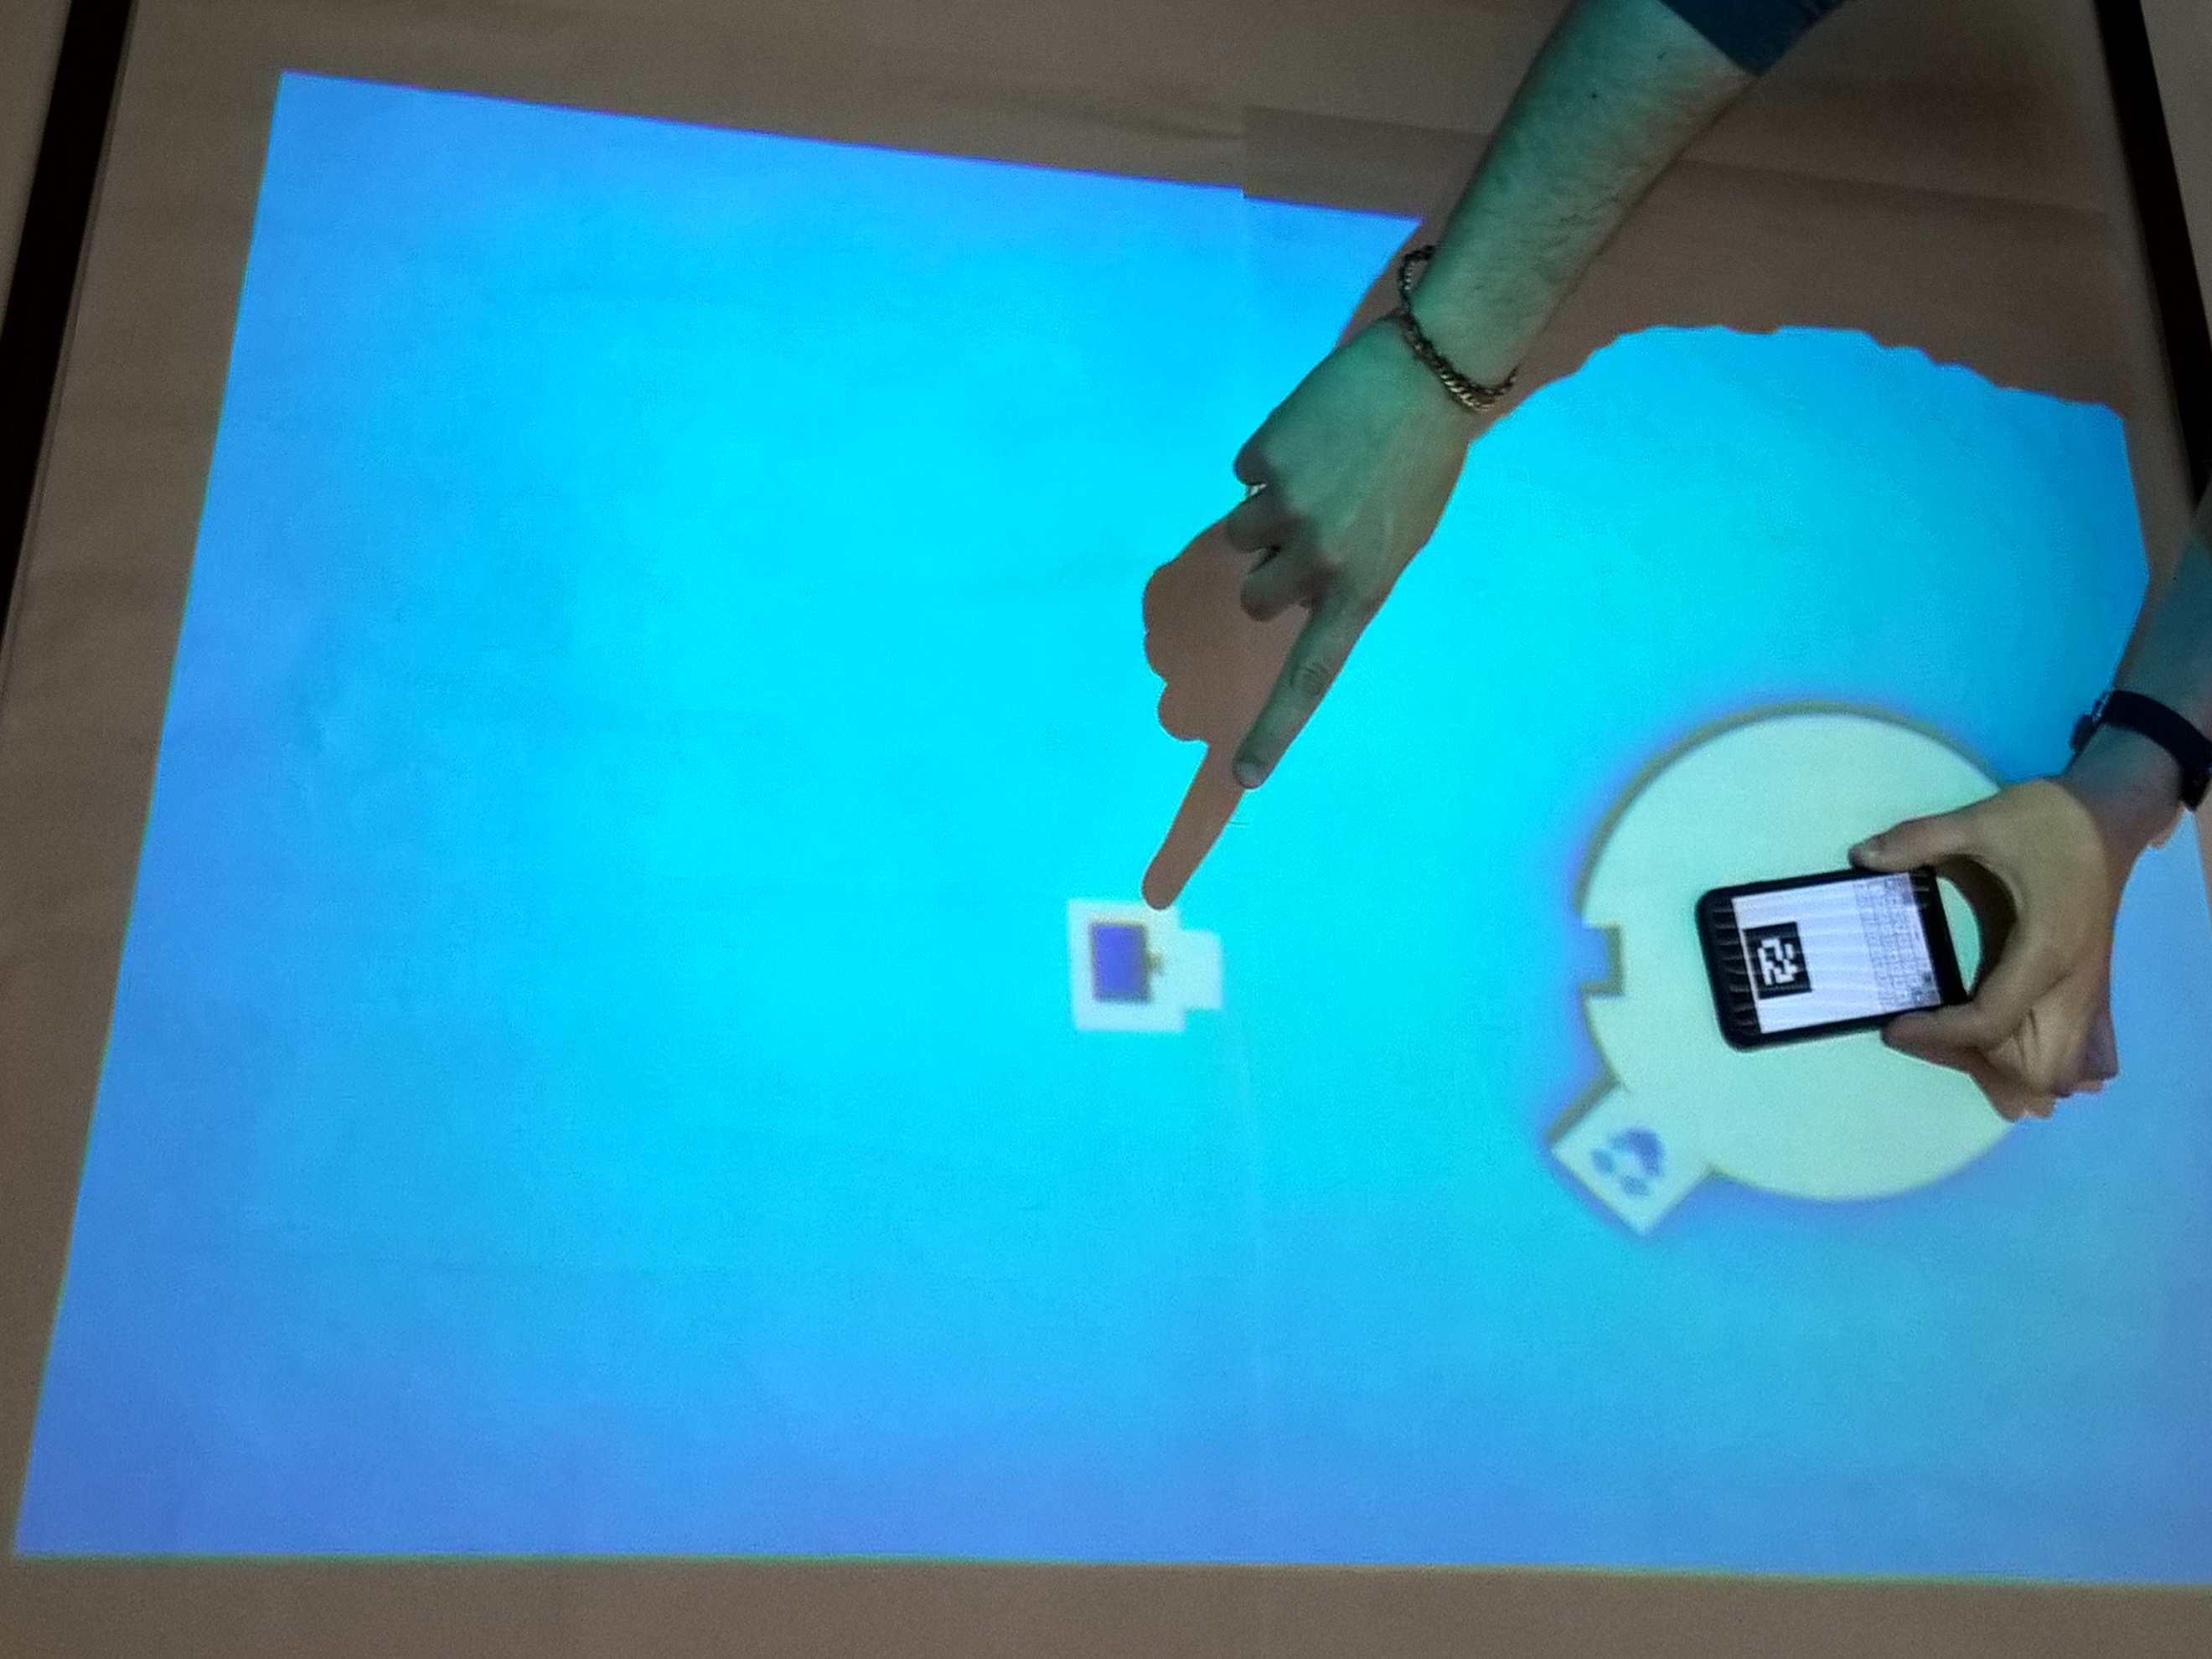
\includegraphics[width=0.7\textwidth]{images/c4/protopic.png}
\caption{An example of a workflow being assembled using \ac{TAPAS}: a keyboard widget is displayed on the smartphone once a new piece requiring an input is assembled.}\label{fig:proto}
\end{figure}

Widgets vary depending on the type of input required: selecting a single option among several will prompt the user with a list box, a single action to be performed will display a button, and a generally unstructured raw text will present a keyboard (figure \ref{fig:proto} and \ref{fig:walkthrough:b}). Once a user enters the requested input on a widget, the latter disappears from the smartphone and the projected halo surrounding it opens up a new hollow to allow for the next piece to be inserted (figure \ref{fig:walkthrough:c}); then using the input, only the hollow that is compatible with it is displayed, aiding users by preventing invalid compositions.

A puzzle piece instance can be added only to one user workflow, but it can be respawned by \ac{TAPAS} later to make it available to other users; all communications through the smartphone and the display are managed via HTTP over the local Wi-Fi network, allowing for network outages.

The features currently available on our prototype, each rendered with a different puzzle piece, are:
\begin{enumerate*}[label=(\arabic*)]
  \item selecting and downloading a file from the user's Dropbox account;
  \item displaying a downloaded PDF file or an image on the main tabletop screen;
  \item searching for a book in the university library and retrieving its location inside the building depicted in an image; and
  \item sending a text document to a specified email address.
\end{enumerate*}

\begin{figure}[ht!] 
  \begin{subfigure}[b]{0.48\linewidth}
    \centering
    \includegraphics[width=0.75\linewidth,trim={800 200 1600 200},clip]{images/c4/TAPAS-1.png} 
    \caption{The first piece is selected and added to the current workflow.}\label{fig:walkthrough:a}
    \vspace{4ex}
  \end{subfigure}\hfill
  \begin{subfigure}[b]{0.48\linewidth}
    \centering
    \includegraphics[width=0.75\linewidth,trim={800 200 1600 200},clip]{images/c4/TAPAS-2.png} 
    \caption{The corresponding widget is displayed on the smartphone's display waiting for user input.}\label{fig:walkthrough:b}
  \end{subfigure}
  \begin{subfigure}[b]{0.48\linewidth}
    \centering
    \includegraphics[width=0.75\linewidth,trim={800 200 1600 200},clip]{images/c4/TAPAS-3.png} 
    \caption{Once the input is inserted, a piece whose input matches the current workflow's output can be added.}\label{fig:walkthrough:c}
  \end{subfigure}\hfill
  \begin{subfigure}[b]{0.48\linewidth}
    \centering
    \includegraphics[width=0.75\linewidth,trim={800 200 1600 200},clip]{images/c4/TAPAS-4.png} 
    \caption{Finally, the workflow is completed and the user can run it from her smartphone.}\label{fig:walkthrough:d}
  \end{subfigure}
  \caption{A step-by-step walkthrough of building a workflow with \acs{TAPAS}.}\label{fig:walkthrough}
\end{figure}

For instance, one could pick 1 and 2 (in this order) and the composed application would download a PDF from the user's Dropbox folder and display its content on the big screen (as depicted in figure \ref{fig:walkthrough}); composing 3 and 2 together would result in looking for an available book in the university library and displaying on the big screen a map depicting its location. These features have been designed with a specific scenario in mind, i.e. providing an interactive public display in an educational space to foster students' interaction on different projects; \acs{TAPAS} has been designed with an open architecture (see figure \ref{fig:arch}) so that new services and corresponding puzzle pieces can easily be added depending on usage scenarios.

Summarizing, our prototype allows users to develop simple workflows while interacting with a \ac{TUI}-based tabletop system installed in public spaces, thus empowering them to adapt and repurpose the latter to their needs.

\section{Study Design}
We evaluated \acs{TAPAS} twice: the first evaluation involved end users in a specific scenario, namely second year university students; they usually share resources with each other and gather information from public displays found within departments' foyers or the library in order to review lectures or complete their coursework. In particular, our participants --- selected among Brunel University second year students in the Department of Computer Science, College of Engineering and Design --- are required to collaborate on a project including many weekly meetings around shared spaces. This presented the right challenge for our application, as the public displays currently available offer services that are only partially relevant and highly scattered for the students' projects and might lead to their interest waning and the under utilisation of such expensive facilities.

Our study allowed us to investigate how \acs{TAPAS} might be employed in such a real-world scenario, i.e. in-the-wild, but also to better define user requirements and ascertain whether they are fully or partially met by our system, informing the following stages of its design. The second  evaluation involved a group of interaction designers and experts and focused on the interaction modality we are proposing with our prototype. The results of both our preliminary studies will be a helpful guide for the redesign of our prototype, even though a fully in-the-wild study is still needed to draw more definitive broad conclusions.

\subsection{User Study}
To get a better understanding of the scenarios where Pervasive Displays might be used, we carried out the first part of our study in a university setting, where many public interactive displays are already being deployed and used; these deployments are not usually effective or adaptable to the multitude of usage contexts they need to deal with and are also affected by the so-called Display Blindness effect \cite{Muller:2009wy}, whereby they are usually overlooked due to people's low expectations of their content value.

\subsubsection{Participants and procedure}
We were interested in investigating the traditional usage contexts of a specific user group --- namely Computer Science undergraduates during their second year --- and how our prototype could help them; as part of their degree, students are clustered into groups of 4-6 and assigned with an Android application project to be undertaken during the course of the year, with the supervision of a teaching staff member, whom they usually meet all together as a group once a week. 

Students are required to meet and work collaboratively every week, normally in the library or in one of the college's meeting rooms, and can use a range of available tools to work together and share information with each other (online dedicated forums or drives, laboratory spaces with coding facilities, etc.). The objective of these meetings is not to develop the Android application --- which is an individual task --- but to coordinate and organize a project plan, eventually designing a Gantt diagram with which students will split the workload into individual tasks. Our study has been conducted partially in-the-wild, since it took place in one of these facilities (a real world setting addressing real world problems) but with a researcher present (partially controlled).

The study involved three groups of students in their second year, made up respectively of four (1 female, 3 males), five (1 female, 4 males) and six (all males) students, reflecting the real project activity requirements and average group size; participants had no prior knowledge of \acs{TAPAS}, but attended their introductory programming course during their first year, thus they already had some programming and problem solving experience. The study was conducted in three different sessions, one for each group; we conducted the study within the University facilities, in a room inside the Department of Computer Science designated to students and staff meetings. Each session lasted one hour and was made up of two consecutive activities (each half an hour long). The first activity addressed the scenario of group project meetings, their current practices and requirements for these. The second activity was a preliminary evaluation of our prototype's feature set and interaction modality. For the latter, we presented the students with \acs{TAPAS} as a ``provotype'' --- i.e., a provocative prototype, namely a prototype that deliberately challenges stakeholders' conceptions by reifying and exposing tensions of existing practice in a context of interest \cite{Boer:2012ku}; this includes a small set of features highly tailored to the evaluation scenario (i.e., university students collaborating with each other), which was the first step in proving our concept. The use of the ``provotype'' was meant to evaluate the current status of the application and especially to elicit the interaction modality requirements that might not have been easily gathered employing only a paper and pencil approach.

\subsubsection{Elicitation of user activities}
During the first activity we asked participants to tell us about the tasks, tools and public resources offered by the University that they would normally use during their weekly gatherings; we provided them with a non-exhaustive sample of icons representing some of the traditional resources and tools they might use, such as books, papers, search engines, smartphones, public display applications and so on. We asked them to place the relevant icons on a sheet of paper, which was divided into 3 different sections: before, during and after the meeting. Participants could use as many icons as they wanted, draw new ones, use post-it notes and link items together. In the end they had to produce an accurate picture of all the activities and tasks usually performed during a meeting and the kind of preparation each one of them requires, as well as all the further activities it might trigger; an example of the final result is depicted in figure \ref{fig:rich}.

\begin{figure}[ht!]
\centering
\fbox{\includegraphics[width=0.85\textwidth]{images/c4/RP.pdf}}
\caption{A snapshot of the rich picture generated by one group participating in our study.}\label{fig:rich}
\end{figure}

The Rich Picture methodology was part of Checkland's Soft Systems Methodology to gather information about a complex situation \cite{146910c69c07485e86a430ed52641409}; Rich Pictures are used before clearly knowing what is to be considered a process and what a structure. They aim at representing a real situation with no constrained ideas. Due to its uncontrolled nature, this methodology is suitable to analyze our in-the-wild scenario, since it is often not easy to clearly separate the processes and structures involved.

Even though there is no specific notation for a Rich Picture and thus they can be misinterpreted, their informality helps communication with users, and might be coupled with an interview and the use of a prototype to allow users to be immersed in the scenario they are modeling \cite{Sutcliffe:2002:URE:581174}. Hence, while building the Rich Picture, we carried out a semi-structured interview in order to control misinterpretations; its results were clustered into \emph{post hoc} generated categories \cite{Pandit:1996um}. We present the categories generated by the interviews in the following:

\paragraph{Scheduling activities} Students use an instant messaging tool to schedule meetings and discuss urgent matters with each other before a meeting, due to its dual real-time and asynchronous nature; they use the same tool to agree on issues to be brought to their supervisor's attention in the next meeting and build a collaborative agenda for it. During their meetings they review upcoming group and single member deadlines and milestones following their tutor's suggestions, storing their progress in each student's logbook, which contains the whole group's progress as well as each member's individual progress. Due to our previous knowledge of student activities our current prototype allows users to access a shared resource, such as their logbook, while giving each one of them a personalized view of their own progress. Nevertheless, from the semi-structured interviews it seems that our prototype will require some form of policy administration on shared-resource editing rights, which will definitely be considered as part of the next iteration of \acs{TAPAS}.

\paragraph{Reporting activities} Each student's logbook also contains a report on the progress made so far; students describe how they have handled completed tasks and report problems they are encountering through the development process that will be then discussed with their tutor. Relevant resources such as papers or books suggested by their tutor or found by individual members are brought to the meeting and shared with the group as a whole or to subgroups (or even with single participants) depending on the scope of their different tasks. Usually only sharing requests are handled during a meeting, leaving actually sending out the resource to the right members as a post-meeting activity, which is subject to mistakes and forgetfulness. Our application allows sharing of resources from one member's private document library to others instantaneously, although thanks to requirements gathering we plan to include in future versions the ability to set groups of users as recipients.

\paragraph{Discussion activities} Discussions happen throughout all the three phases: before and after the meeting students use instant messaging tools to discuss pressing issues they came across during the development, or email for longer and more detailed discussions, seeking advice and suggestions from their peers. During the meeting itself the group discussion mainly focuses on issues relevant to all the members rather than individuals, but it may occasionally involve subgroups working on similar tasks. Using the large tabletop screen those requirements are naturally met by our prototype. Due to its collaborative features, it can be used to show all the other members some interesting resource and thus foster discussion among members of a groups. The prototype also makes it easy to hold multiple discussions between different subgroups.

\subsubsection{Elicitation of interaction modalities}
After the first activity (gathering requirements), we then proceeded with the second activity (30 minutes long) by briefly introducing the current version of \acs{TAPAS} to participants, explaining to them how the system works. We then let them play with it for 15 minutes (figure \ref{fig:studs}), and finally carried out a semi-structured interview --- mainly focused on the proposed interaction modality. We reminded them that our objective for this activity was to elicit the interaction modalities requirements that might not easily have been gathered just by employing a Rich Picture approach.

Results point out how \acs{TAPAS} offers a quite satisfactory user experience; as expected, students' feedback mostly focused on missing features and the interaction with the system.

Each group managed to successfully assemble (at least once) two workflows: the first one started with downloading a PDF file from a Dropbox account and displaying a preview on the main tabletop surface, while the second one started with looking for a specific book in the university library and depicting its location on the main screen. One group even assembled a more complex workflow, consisting of the download of a text file from Dropbox and its subsequent dispatch via email to an address they chose. Indeed, all these three workflows might come in handy during a students' meeting, according to the Rich Picture's results: the first two workflows belong to the ``Discussion activities'', and the third one to the ``Reporting activities''.

From the feedback we have obtained it is clear how a \ac{TUI} is an easy and effective way of interacting with the system throughout the composition of a workflow. Even though all our participants are Computer Science undergraduates, their second-year group project is their first chance of tackling a wider problem solving scenario, unlike their first year's individual development of smaller applications. This more complex project required them to learn abstraction and decomposition skills, whilst collaborating with peers. Using the puzzle metaphor and workflows together with tangible interaction seemed to help them build the required Computation Thinking skills: for instance, collaboratively planning and designing the application's tasks and assigning them to each participant seems like a suitable scenario to practice abstraction and composition skills. Moreover, as with API development, the recipe metaphor provides different levels of transparency and abstractions useful to generalize the problem whilst assembling a puzzle might help with decomposing a bigger problem into smaller ones \cite{Wing:2008cv}.

Nonetheless, the feedback showed that tangible interaction is not very ``natural'' when it comes to manipulating their output: every participant trying out the prototype attempted to move images displayed on the screen with their fingers, suggesting that manipulating items through objects might feel ``natural'' only when operating in composition/developing mode, and not when there is actual content the user needs to directly manipulate available on the screen. This follows directly from our choice of employing a \ac{PbI} paradigm, which uses a syntactic construct to specify a workflow's instructions as opposed to exploiting only contextual actions on resulting artifacts --- i.e., \ac{PbD}. 

From the interaction point of view we noticed one interesting remark made by one of the participants: continuously tracking the smartphone's position on the surface using a fiducial marker requires the user to not cover its display with her hand when moving it; however, the user's hand position on the smartphone might depend on her posture: if the user is standing straight, it feels more ``natural'' to hold it from above --- thus covering the fiducial marker with her palm --- while if sitting down, the user might feel more comfortable grabbing it from the side, without covering its display, allowing its movements to be tracked. Because the majority of existing smartphones are shaped in the same way, it is worth studying this effect in more detail, in order to establish whether we could provide users with a physical enclosure affording the ``right'' way of holding the smartphone or whether it is a negligible effect when the system runs on horizontal displays of a certain distance from the floor.

\begin{figure}[ht!]
\centering
\includegraphics[width=0.7\textwidth]{images/c4/studs.png}
\caption{One of the participating groups to our study working with \ac{TAPAS}.}\label{fig:studs}
\end{figure}

Summarizing, we gathered several detailed scenario requirements from users in the form of three usage contexts, which targeted scheduling, reporting and discussion activities; we highlighted how the current version of \acs{TAPAS} deals with them and how we are going to address those that are not yet satisfied. The same users appear to cope easily with \ac{TAPAS}' interaction modality during the workflow editing phase, but we will need to devise a different interaction style when it comes to manipulating their results.

\subsection{Designer Study}
We also interviewed three interaction design experts to get feedback on the modality we have implemented in \acs{TAPAS}; we carried out the interviews in a controlled environment (figure \ref{fig:des}), namely during a workshop on the island of Tiree, during the bi-annual Tiree Tech Wave, a gathering of experts in various fields, ranging from interaction designers and artists to computer scientists. The study involved simultaneously two HCI experts and a product designer and lasted 45 minutes. We briefly introduced our prototype to them, explaining the rationale behind its design and the scenarios we are targeting; then we gave them a demonstration of how it works, going through some examples of its usage in a real world scenario. Finally we carried out a semi-structured interview focusing on the strengths and weaknesses of our prototype in relation to the interaction modality and its applicability in-the-wild, more precisely covering the easiness of the puzzle metaphor, the use of smartphones as tangible objects, possible application scenarios and future features.

Designers liked the overall idea and the personalization approach for Pervasive Display scenarios, namely using a smartphone as a tangible instead of just a passive object to identify users and link their personal information with the movements they perform on the very same device. In particular, they liked the puzzle metaphor since it looked a straightforward way of understanding the composition of workflows to address users' needs.

\begin{figure}[ht!]
\centering
\includegraphics[width=0.7\textwidth]{images/c4/tiree.png}
\caption{The designer study setting.}\label{fig:des}
\end{figure}

They recognized the potential of such a system in public spaces, due to its ease of deployment and the cheapness and high availability of the technologies involved: thanks to the simple architecture, \acs{TAPAS} allows deployment in any digitally augmented surface just by installing an RGB camera and running the application on a production server; it can be left in public spaces for a long period of time without the need to perform mundane maintenance operations aimed at adding new features, since users are empowered to repurpose it themselves.

Some of their suggestions focused on the way \acs{TAPAS} presents data to users and the use of the dynamic widget to get some input from them: due to the kind of data handled right now --- namely lists of files within directories or book titles in a database --- it makes sense to prompt users to choose an option from a list or offer a keyboard to input raw text. Nevertheless, this will not be the case if we have to deal with more structured data types, such as points of interest on a map: therefore, they suggested that due to the complexity of workflows that might be put together by final users, widgets might be designed to be more flexible and personalizable depending on the two-fold level of interaction between the user perspective and data perspective related to the specific data handled by the widget. They emphasized that the two perspectives are interlinked and reinforced mutually. We propose to consider elements of human-centered information visualization in the redesign of the widgets for the next interaction prototype; for instance, by following visual metaphors that incorporate semantic relationships of visual objects both in the physical (tangible) and virtual (digital) world \cite{Majumder:2013wt,Bigelow:2014th}.

Furthermore, interviewees pointed out how this continuous back and forth movement, between interacting with the smartphone to input data and with the large display to assemble workflows, might be confusing for users: interacting with two different devices, each one with a different interaction style --- i.e. tangible on the tabletop, multi-touch on the smartphone --- and different underlying metaphors, requires a relatively high cognitive effort in constantly switching paradigm and some users might also miss what is happening on one device while they are too focused on interacting with the other. That is why interviewees suggested keeping the tabletop as the main interaction focus by providing a mixed interaction modality: moving the smartphone will still be used to assemble the puzzle pieces but once one of them requires a certain input, the widget will appear on the tabletop surface --- close to it --- and the user will interact with it using her fingers.

The final observation concerns the puzzle metaphor we are using: although it appears to be quite an easy to grasp concept, we might need to offer some additional visual cues to improve its efficacy; interviewees suggested that in addition to shapes to indicate functions compatible with the currently generated output, we might highlight the available ones and darken the incompatible ones, even when the former are not available due to network outages or other problems; or associate colors to shapes.

Indeed, there are clearly positive elements in our design for \ac{EUD} of workflows to adapt public display services to users' needs, such as the puzzle metaphor, the use of the smartphone as being tangible and personal, and the ease of prototype deployment in-the-wild due to its low-cost and flexible architecture. Nonetheless, there are some major challenges to be addressed in future in terms of interaction design requirements, such as the flexibility/programmability of widgets and improving the puzzle metaphor to highlight available functionalities.

\section{Results}

\section{Discussion}
From our study we identified two relevant challenges in the field of Tangible Programming on public interactive displays: the first stems from our user study with students and is about the duality of composing workflows and executing workflows in tangible environments; the second challenge has emerged during the study with designers and is related to the use of Visual Languages in the domain of Tangible Programming. 

The user experience seems to differ when the tangible interaction is used for composing services with the puzzle metaphor (positive experience) from when they interact and collaborate on the results of the workflow execution through their smartphones (less positive experience). This could be due to the different set of constructs involved within each stage:

\begin{enumerate}
\item Building a workflow requires the user to deal with abstract concepts --- like functions and constraints --- that are not naturally coupled with any existing physical counterpart; providing users with an intuitive metaphor (the puzzle) and enabling them to interact with the system in a natural way (through a tangible) might be an effective strategy to help them build the right mental model, together with exposing the right transparency level of the workflows' inner logic in order to improve abstraction and decomposition skills, indeed helping to develop their Computational Thinking abilities. 

\item In a \ac{NUI} based environment, direct manipulation of contents is more intuitive than using intermediate control mechanisms; hence, when it comes to manipulating results produced by their workflows, users require the interface to be completely transparent, without any syntactical --- least of all tangible --- artifact to operate on an environment's constructs. 
\end{enumerate}

This contrast is also evident from the literature (see section \ref{tp}) highlighting the many differences between the \ac{PbD} and \ac{PbI} paradigms: due to its very nature, when a system exploits \ac{PbD}, the composition and execution environments are perfectly overlapped, i.e. the same artifacts the users operate on to program the system are used also to interact with its results, as with Robot Programming by Demonstration; in Robot Programming by Demonstration users teach movements to a robot by simply simulating them directly onto its body. This is radically different from a \ac{PbI} approach, where the two environments --- composition and execution --- are generally detached from one another, each one using different metaphors and concepts, e.g., in Yahoo! Pipes there is a visual editor for composing a pipe (data-flow) that generates a specific execution environment made of \ac{GUI} elements as designed by the user. While this distinction might be overlooked from an interaction perspective when a system only relies on a \ac{GUI}, it becomes more relevant when it is about \acp{TUI}. Even though \ac{PbI} seemed the right paradigm to choose in our scenario due to its generalizability and the benefits brought to Computational Thinking skills, we argue that choosing the right paradigm according to the naturalness of interaction is clearly scenario-dependent, as is often the case with Domain Specific Visual Languages.

From the second study with designers an interesting challenge has emerged which is related to the use of Visual Languages with \acp{TUI}. In particular, we have noted that the majority of examples we found in the literature (see section \ref{tp}), including our prototype, use Visual Languages when employing a \ac{PbI} paradigm. 

Visual Languages have been widely used within the field of \ac{EUD} in order to ease the development process for end users; the interaction paradigm used for Visual Languages is \ac{GUI}-based, whilst due to our scenario, i.e. Pervasive Displays, a more natural way of allowing \ac{EUD} would be to support Tangible User Interaction. One challenge would be to study whether there is an \ac{EUD} paradigm more suitable for \ac{TUI} environments: this challenge would require understanding whether any of the available paradigms, e.g., \ac{PbI} and \ac{PbD}, are suitable for Tangible Programming or if --- on the contrary --- new paradigms need to be introduced. There is some evidence, as in Robot Programming by Demonstration for instance, that \ac{PbD} is suitable for that specific scenario using Tangible Programming but, as often happens in the \ac{EUD} community, the solution might be domain dependent.

A final remark concerns the problem we were investigating first, namely fostering the long-term appropriation of Pervasive Displays by enabling users to repurpose them through \ac{EUD}: during our first study we collected and clustered the requirements of a typical scenario where Pervasive Displays could already be used, but --- due to their maintenance issues and progressive loss of interest by users --- are not yet widespread. Our analysis reported three types of activities that end users need to be able to carry easily out with a Pervasive Display in order to properly support user needs in the scenario we considered:
\begin{enumerate*}[label=(\arabic*)]
  \item scheduling,
  \item reporting,
  \item and discussion activities.
\end{enumerate*}

While ours was indeed just a preliminary study on a specific application domain, we can certainly use its findings to highlight some of the issues preventing Pervasive Display deployment in-the-wild for long periods of time. Supporting collaboration is definitely a much needed feature, both peer-to-peer --- that is where all participants have the same role within the group (e.g., discussion activities) --- and chaired modes (e.g., reporting activities); discovering user roles is the cornerstone, and the use of smartphones can definitely come in handy \cite{Clinch:2013uj}. Moreover, Pervasive Displays need to support users in individual activities as well (e.g., scheduling activities), enabling them to use their preferred tools while carefully considering the resulting privacy issues; indeed, our choice of employing smartphones as tangible probes in \acs{TAPAS} was influenced by privacy concerns, allowing us to draw upon user data while keeping the user in control of what she wants to share and with whom. For this reason, we are currently working on the \acs{TAPAS}' web app in order to develop a more sophisticated interface that enables users to effectively tweak their privacy settings and control which data \acs{TAPAS} can have access to.

Finally, as we previously stated, it is undoubtedly worth pointing out the shortcomings of our studies: the limited number of components developed and deployed to the system prevented us from fully evaluating its usage in a real in-the-wild scenario, thus our findings cannot be properly generalized for many other contexts. Yet, since we employed \acs{TAPAS} as a provotype --- that is to challenge users by exposing tensions and thus to support design explorations \cite{Boer:2012ku} --- observations related to the interactions users and designers carried out can give us a good insight into its real usage. Moreover, a fully in-the-wild study is needed to properly highlight how \acs{TAPAS} relates to mundane Pervasive Displays activities.

\section{Conclusion}
A fairly recent trend in the Pervasive Displays research area is to design long-term in-the-wild deployments outside controlled laboratory settings and without any researcher supervision; nevertheless, these deployments present two main drawbacks: the first is the expensive setup and maintenance and the second is the progressive loss of interest shown by users, due to the lack of new features satisfying their shifting needs. A way of tackling this problem is to allow users to adapt the system themselves without the intervention of the site managers.

In this paper we introduced \acs{TAPAS}, an application running on a Pervasive Display system, which allows users to adapt and repurpose the system using their smartphones combining a tangible and visual interaction. We have detailed its architecture and highlighted the advantages and rationale behind its design following a workshop with experts, making the case for the ease and convenience of its in-the-wild deployment.

We evaluated \acs{TAPAS} by carrying out a two-phase study, the first phase involving end users in a specific scenario --- second year undergraduates working in groups --- and the second phase with interaction designers. From the first study's results, it seems that our prototype provides a positive user experience and could be used in a collaborative project scenario where people work together to tackle a complex problem; a potential side effect caused by employing our prototype might be a development of Computational Thinking skills, thanks to our design rationale. However, from our findings it also appears that coupling tangible interaction with a \acl{PbI} paradigm causes an incompatibility of interaction styles between the composition and the execution environments, where the use of a different tangible-based syntactic construct in the former causes the need for a different interaction style to be used in the latter.

The second study we conducted to evaluate our prototype was focused on its interaction modality and involved a group of interaction design experts; the results show that participants liked the proposed interaction style, recognizing the potential of the exploited puzzle metaphor in easing the adaptation tasks for the end users. They also suggested extending the platform in order to cope with more complex data to be manipulated by end users. However, from the results it seems that exploiting Visual Languages within a \acl{TUI} system might not be the best way of providing users with a natural interaction experience, thus further investigations are needed to determine the role of the scenario in the choice of the right paradigm (i.e. \acl{PbI} or \acl{PbD}).

In the future we plan to study in more detail issues arising from our findings, with particular attention to the main challenges discussed in section \ref{sec:disc}. We plan to exploit the feedback obtained from our studies in the next iteration of \acs{TAPAS}' design and carry out additional evaluation studies in other public scenarios, such as university settings or urban areas, and in non-public collaborative contexts too, e.g., within a company. Moreover, further studies will be carried out in order to draw more definitive conclusions regarding the effect of the proposed interaction modality on the development of Computational Thinking skills, as well as within a fully in-the-wild setting, where participants will be prompted to use the system without any researchers' intervention. We also plan on studying whether extending \acs{TAPAS}' functionalities without support for more complex workflows, as suggested by designers and users, might improve its adoption.